\documentclass[9.5pt]{beamer}

\mode<presentation>
{
  \usetheme{Warsaw}       % or try default, Darmstadt, Warsaw, ...
  \usecolortheme{default} % or try albatross, beaver, crane, ...
  \usefonttheme{serif}    % or try default, structurebold, ...
  \setbeamertemplate{navigation symbols}{}
  \setbeamertemplate{caption}[numbered]
} 

\usepackage[utf8]{inputenc} % accents 8 bits dans le fichier
\usepackage[T1]{fontenc}      % accents codés dans la fonte
\usepackage[french]{babel}
\usepackage{amsmath,amssymb}
\usepackage{graphicx}
\usepackage{fancyhdr}
\usepackage{siunitx}
\usepackage[mode=buildnew]{standalone}
\usepackage{algorithmicx}
\usepackage{algorithm}
\usepackage{algpseudocode}


% Here's where the presentation starts, with the info for the title slide
\title[MPNA : MIS]{Présentation MPNA \\Méthode des itérations simultanées}
\author[\bsc{Beaupère} \& \bsc{Granger}]{Matthias \bsc{Beaupère} \& Pierre \bsc{Granger}}
\institute{M2 CHPS}
\date{\today}

\begin{document}
\setbeamercolor{captioncolor}{fg=white,bg=red!80!white}
\setbeamertemplate{caption}{%
\begin{beamercolorbox}[wd=0.8\linewidth, sep=.2ex]{captioncolor}\tiny\centering\insertcaption%
\end{beamercolorbox}%
}

\begin{frame}
  \titlepage
\end{frame}

\begin{frame}{Plan}
	\tableofcontents[hideallsubsections]
\end{frame}

\section{Introduction}
	\begin{frame}{Introduction}

	\end{frame}

\section{Présentation de l'algorithme}
	\begin{frame}{La méthode des itérations simultanées}

	\end{frame}

\section{Séquentiel}
	\subsection{Description}
		\begin{frame}{Données d'entrée}
			\begin{itemize}
				\item $M$ : taille du sous-espace de Krylov
				\item $k$ : nombre de vecteurs propres demandé
				\item $p$ : précision demandé
				\item $A$ : matrice de taille $N\times N$ donnée en entrée
				\item $N_{iter}$ : nombre d'itérations
			\end{itemize}
		\end{frame}
		\begin{frame}{Description de l'algorithme}
			\begin{algorithmic}
				\State $Q \gets rand()$
				\While {$i = 0 .. N_{iter}-1$ OU max(precisions) < p}
					\State $Z = AQ$
					\State Gram-Schmidt $Q$
					\State Projection $B = Z^tAZ$
					\State Décomposition de Schur $B = Y^tRY$
					\State Retour dans l'espace d'origine $Q = ZY$
					\State Calcul de la précision des vecteurs de $Q$
					\State Sélection des $k$ vecteurs propres
				\EndWhile
			\end{algorithmic}
		\end{frame}

	\subsection{Performances théoriques}
		\begin{frame}{Performances théoriques}
			\begin{tabular}{ l l }
				Produit $AQ$ & $O(N^2M)$ \\
				Gram-Schmidt & $O(NMlog(M))$ \\
				Projection & $O(N^2M)$ \\
				Décomposition de Schur & $O(1)$ \\
				Précision & $O(NM^2)$ \\
				Sélection & $O(1)$ \\
			\end{tabular}

			
			$$
			\fbox{$C^{tot} = O(N_{iter}N^2M)$}
			$$
		\end{frame}

	\subsection{Performances pratiques}
		\begin{frame}{Nombre d'itérations}
			\begin{figure}
				\centering
				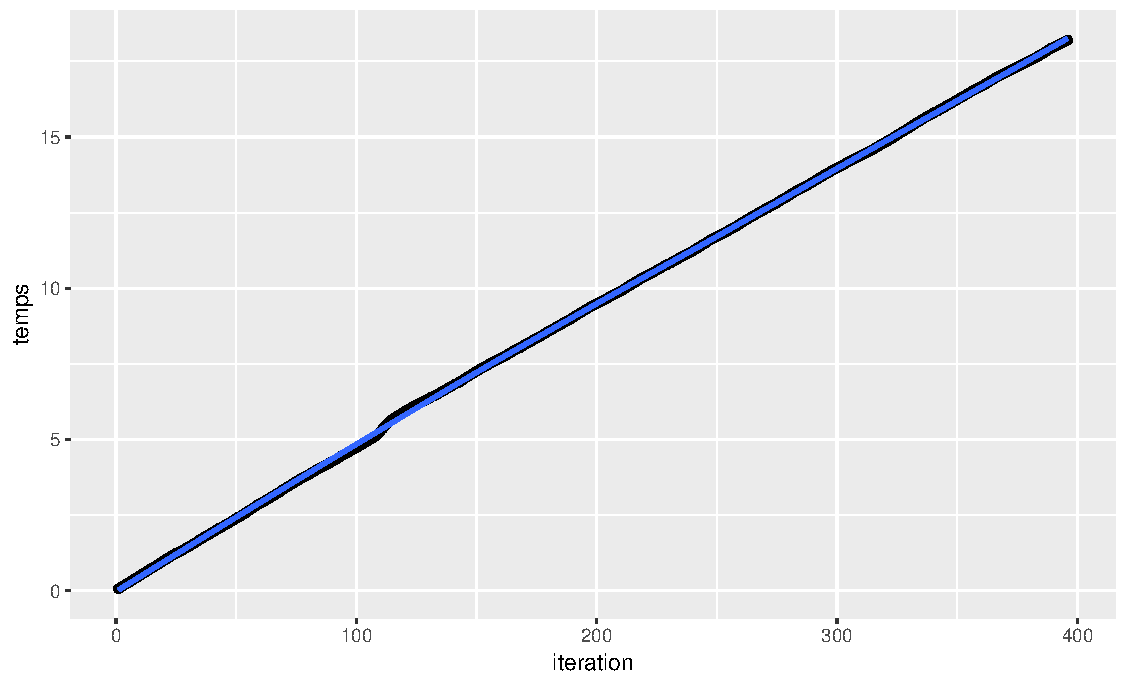
\includegraphics[width = 0.7\linewidth]{../rapport/plots/tvsiter.pdf}
				\caption{Evolution du temps de calcul en fonction du nombre d'itérations. \label{fig:tvsiter}}
			\end{figure}
		\end{frame}

		\begin{frame}{Taille du sous-espace de Krylov $m$}
			\begin{figure}
				\centering
				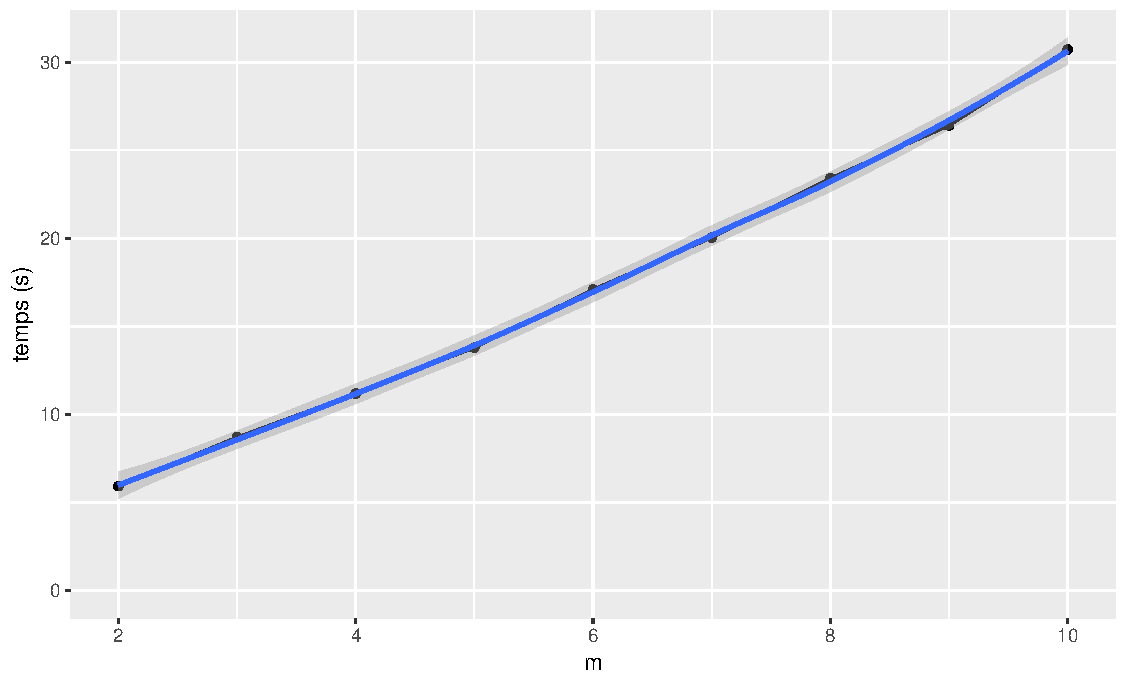
\includegraphics[width = 0.7\linewidth]{../rapport/plots/tvsm.pdf}
				\caption{Evolution du temps de calcul en fonction de la taille du sous-espace de Krylov $m$. \label{fig:tvsm}}
			\end{figure}
		\end{frame}

		\begin{frame}{Taille de la matrice $M$}
			\begin{figure}
				\centering
				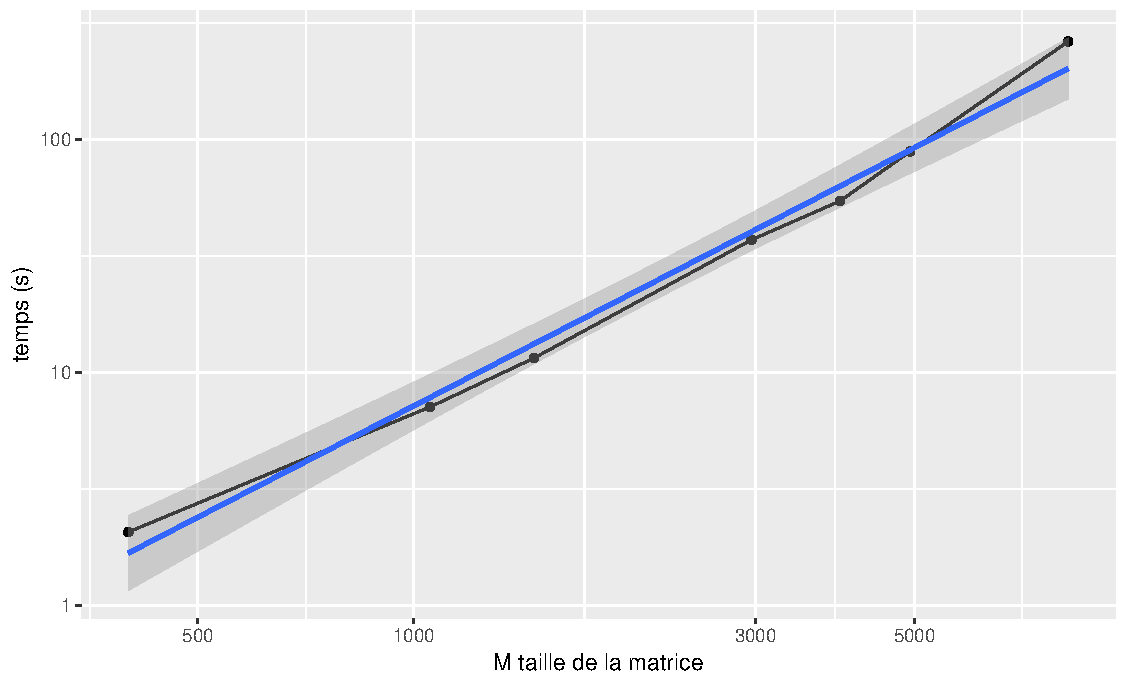
\includegraphics[width = 0.7\linewidth]{../rapport/plots/tvsM.pdf}
				\caption{Evolution du temps de calcul en fonction de la taille de la matrice $M$. \label{fig:tvsM}}
			\end{figure}
		\end{frame}

	\subsection{\'Etude de convergence}
		\begin{frame}{Influence de $m$}
			\begin{figure}
				\centering
				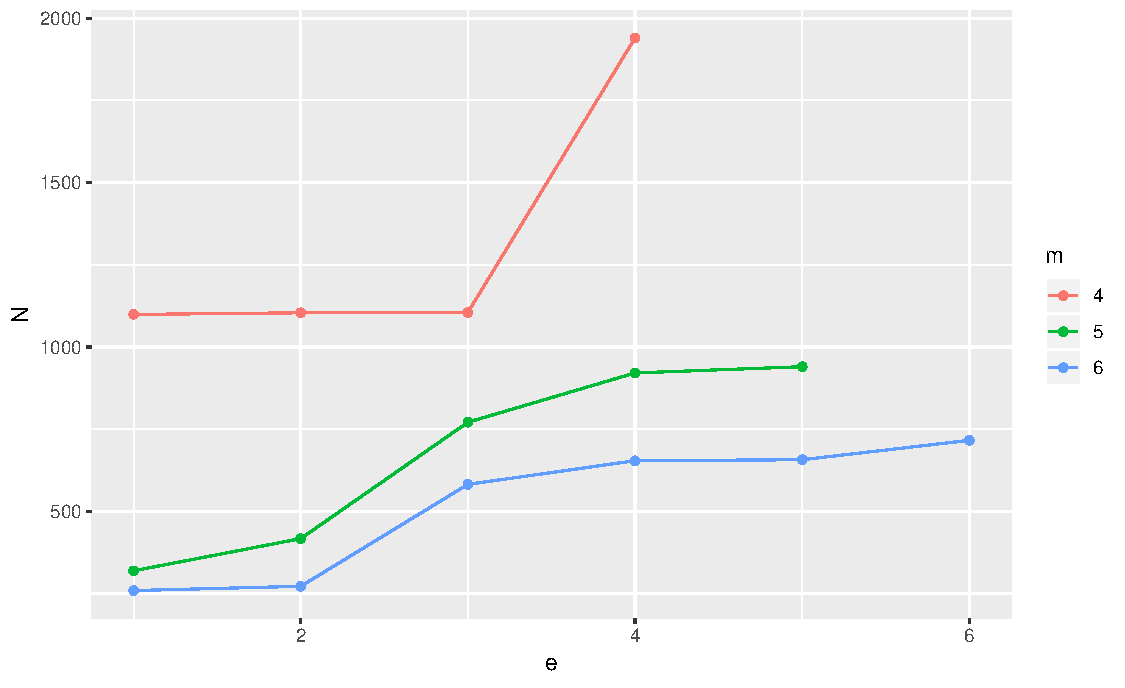
\includegraphics[width=0.8\linewidth, keepaspectratio]{../rapport/plots/Nvse-m_p6.pdf}
				\caption{Nombre d'itérations $N$ nécessaires pour faire converger $e$ valeurs propres pour différentes tailles de sous-espace de Krylov $m$ et une précision $p=\SI{e-6}{}$ \label{fig:Nvse-m_p6}}
			\end{figure}
		\end{frame}

		\begin{frame}{Influence de $p$}
			\begin{figure}
				\centering
				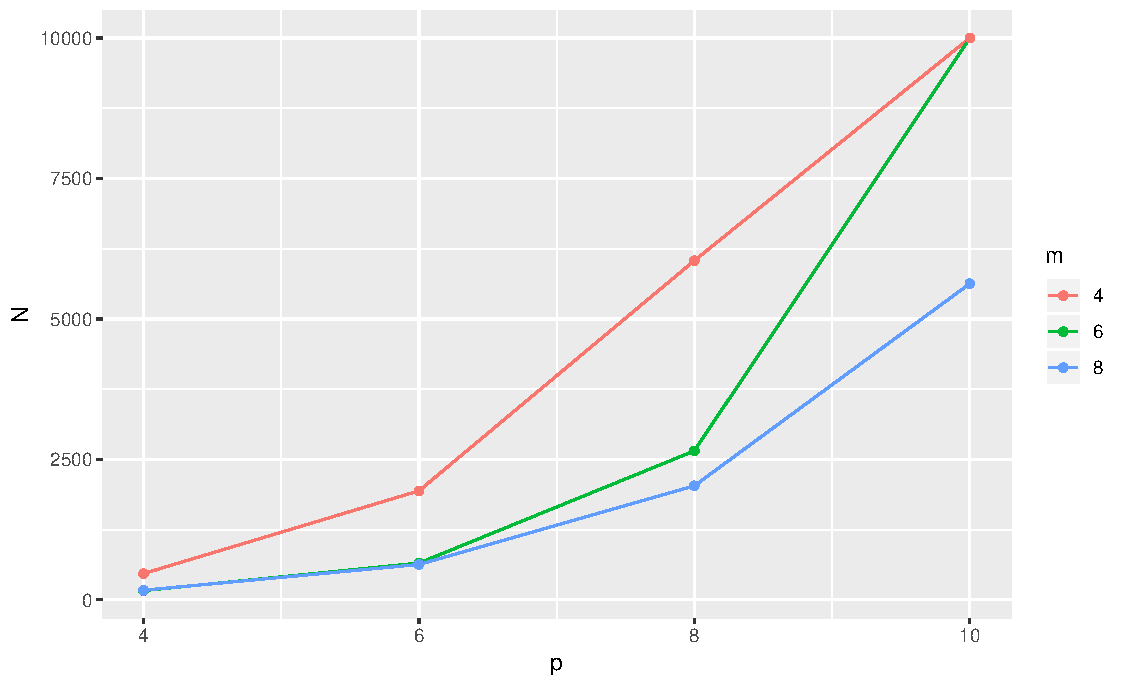
\includegraphics[width=0.8\linewidth, keepaspectratio]{../rapport/plots/Nvsp-m_e4.pdf}
				\caption{Nombre d'itérations $N$ nécessaires pour faire converger $e = 4$ valeurs propres pour différentes tailles de sous-espace de Krylov $m$ et une précision $p$ \label{fig:Nvsp-m_e4}}
			\end{figure}
		\end{frame}

	\subsection{Locking}
		\begin{frame}{Principe du locking}
			\begin{block}{Justificatons}
				\begin{itemize}
					\item Vitesses de convergence différentes des vp.
					\item Perte de temps.
					\item Instabilités numériques.
				\end{itemize}
			\end{block}

			\begin{exampleblock}{Le locking}
				\begin{itemize}
					\item On verrouille les vp lorsqu'ils ont convergé.
					\item On ne le multiplie par A.
					\item On diminue m.
					\item On l'utilise pour l'orthonormalisation.
				\end{itemize}
			\end{exampleblock}
		\end{frame}

		\begin{frame}{Performances du locking}
			\begin{figure}
				\centering
				\begin{columns}
					\column{0.5\linewidth}
					\centering
					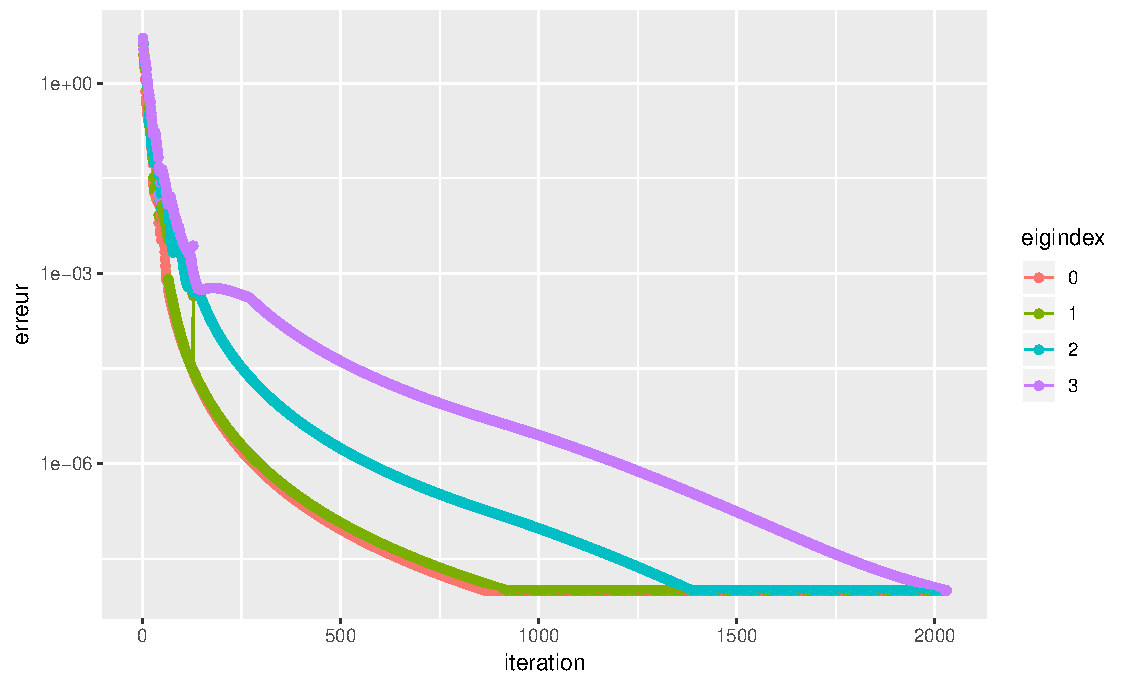
\includegraphics[width=\linewidth, keepaspectratio]{../rapport/plots/wlock_e4_p8_m8.pdf}
					\caption{Avec locking\label{wlock_e4_p8_m8}}

					\column{0.5\linewidth}
					\centering
					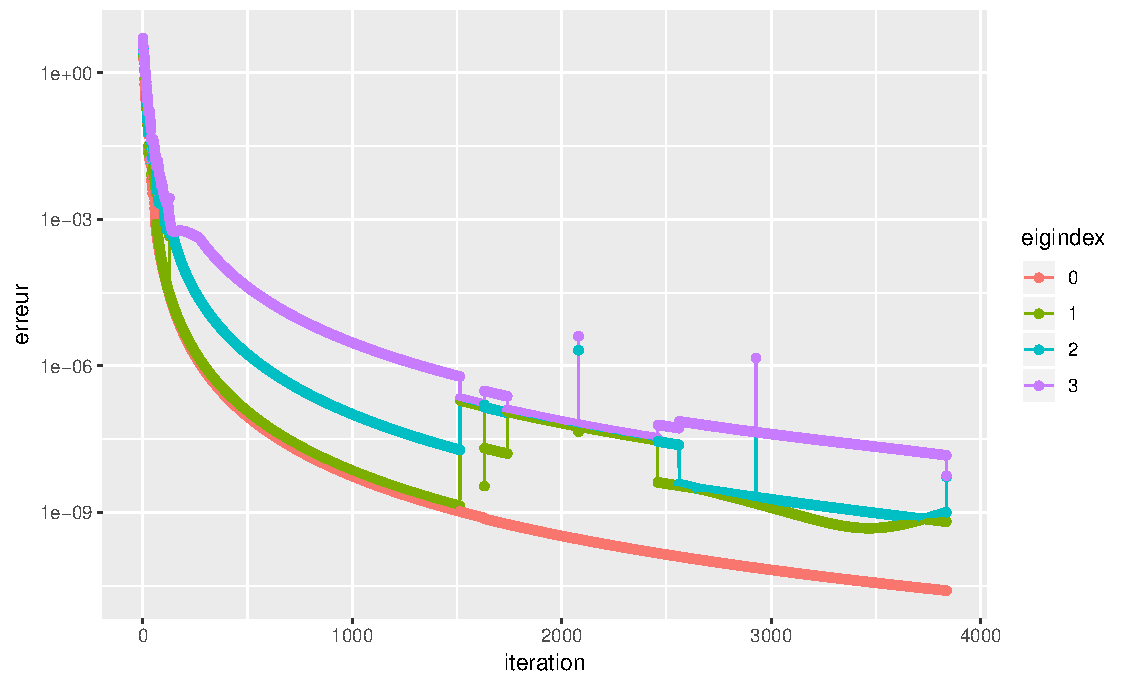
\includegraphics[width=\linewidth, keepaspectratio]{../rapport/plots/wolock_e4_p8_m8.pdf}
					\caption{Sans locking\label{wolock_e4_p8_m8}}
				\end{columns}
				\caption{Précision au cours des itérations $N$ pour $e = 4$ valeurs propres pour une taille de sous-espace de Krylov $m=8$\label{fig:comp_locks}}
			\end{figure}
		\end{frame}

		\begin{frame}{Performances du locking}
			\begin{figure}
				\centering
				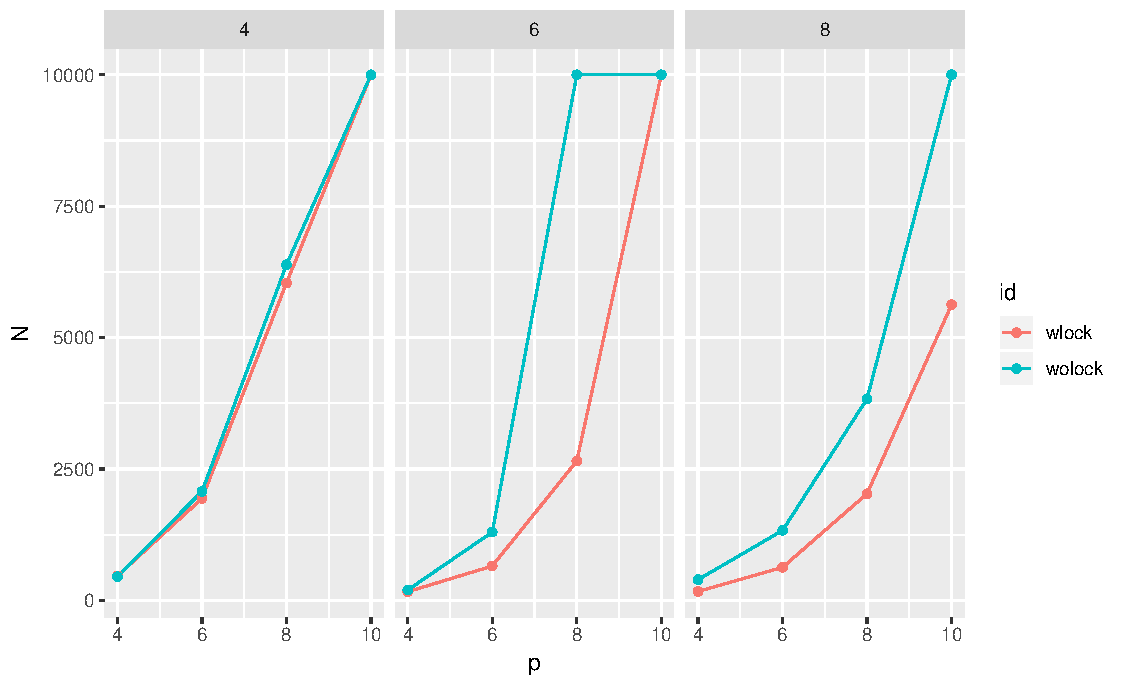
\includegraphics[width=0.8\linewidth, keepaspectratio]{../rapport/plots/Nvsp_complock.pdf}
				\caption{Nombre d'itérations $N$ nécessaires pour faire converger $e = 4$ valeurs propres pour différentes tailles de sous-espace de Krylov $m$ et une précision $p$ avec et sans utilisation du locking \label{fig:Nvsp_complock}}
			\end{figure}
		\end{frame}

\section{Multic\oe{}urs}
		\subsection{Description}
		\begin{frame}{Multic\oe{}urs}

		\end{frame}

	\subsection{Performances théoriques}
		\begin{frame}{Multic\oe{}urs : performances théoriques}

		\end{frame}

	\subsection{Performances pratiques}
		\begin{frame}{Multic\oe{}urs : performances pratiques}

		\end{frame}

\section{Multin\oe{}uds}
	\subsection{Description}
		\begin{frame}{Multin\oe{}uds}

		\end{frame}

	\subsection{Performances théoriques}
		\begin{frame}{Performances théoriques}

		\end{frame}

	\subsection{Performances pratiques}

		\begin{frame}{Multin\oe{}uds : performances pratiques}

		\end{frame}

\section{Conclusion}
	\begin{frame}{Conclusion}

	\end{frame}

\end{document}
